\documentclass[mathserif]{beamer}
\usepackage{beamerthemeshadow}
\usepackage{beamerthemesplit}
%\usetheme{shadow}
\usecolortheme{default}
\setbeamertemplate{footline}[frame number]
\useinnertheme[shadow=true]{rounded}
%\setbeamertemplate{footline}{\insertframenumber/\inserttotalframenumber}
%\useoutertheme{infolines}
%\setbeamertemplate{headline}{} % removes the headline that infolines inserts

%\usetheme{boxes}
%\usepackage{amsmass}
%\usepackage{amssymb,amsfonts,url}

\usepackage{algorithm}
\usepackage{algorithmic}

\usepackage{graphicx}
\graphicspath{{Problems/}}

%\usepackage{CJK}
%\usepackage{pinyin}

%    \begin{figure}
%        \centering
%        \includegraphics[width=0.8\textwidth]{newGeneRep.eps}
%    \end{figure}

% \begin{figure}%
%   \begin{center}%
%     \begin{minipage}{0.70\textwidth}%
%      \includegraphics[width=1.0\textwidth]{comp25000.eps}%
%     \end{minipage}%
%     \begin{minipage}{0.30\textwidth}
%      \includegraphics[width=1.0\textwidth]{comparelabel.eps}%
%     \end{minipage}%
%   \end{center}
% \end{figure}

% \begin{table}
%   {\begin{tabular}{l|rrr}\hline
%       & \multicolumn{3}{c}{Actual number of DCJ operations}\\
%       \# genes &\# genes $\times 1$&\# genes $\times 2$&\# genes  $\times 3$ \\
% \hline
%      (a)~25,000 & 0.5\% ~~&  0.9\% ~~& 1.7\%~~\\
%       (b)~10,000 & 0.8\%~~ &  1.4\% ~~& 2.7\%~~\\
%      (c)~ 1,000 & 2.7\%~~ & 4.7\%~~ & 14.7\%~~\\ \hline
%     \end{tabular}} {}%
% \end{table}

% \begin{eqnarray}
% T(n) &=&  \sum\nolimits_{i=1}^n C_i \\
%      &=&  \# PUSH + \#POP \\
%      &<& 2\times \#PUSH \\
%      &<& 2n \\
% \end{eqnarray}

% \[ 
% \begin{matrix}
% \begin{pmatrix}
% C_{11} & C_{12} \\ 
% C_{21} & C_{22} 
% \end{pmatrix}
% =
% \begin{pmatrix}
% A_{11} & A_{12} \\ 
% A_{21} & A_{22}  
% \end{pmatrix}
% 
% \begin{pmatrix}
% B_{11} & B_{12} \\ 
% B_{21} & B_{22}  
%  
% \end{pmatrix}
%     
%    \end{matrix}
% \]
% 
% 
% \begin{eqnarray}
%  C_{11} &=& (A_{11}\times B_{11}) + (A_{12} \times B_{21}) \\
% C_{12} &=& (A_{11}\times B_{12}) + (A_{12} \times B_{22}) \\
% C_{21} &=& (A_{21}\times B_{11}) + (A_{22} \times B_{21}) \\
% C_{22} &=& (A_{21}\times B_{12}) + (A_{22} \times B_{22}) 
% \end{eqnarray}
% \begin{figure}%
%      \begin{minipage}{0.32\textwidth}%
%       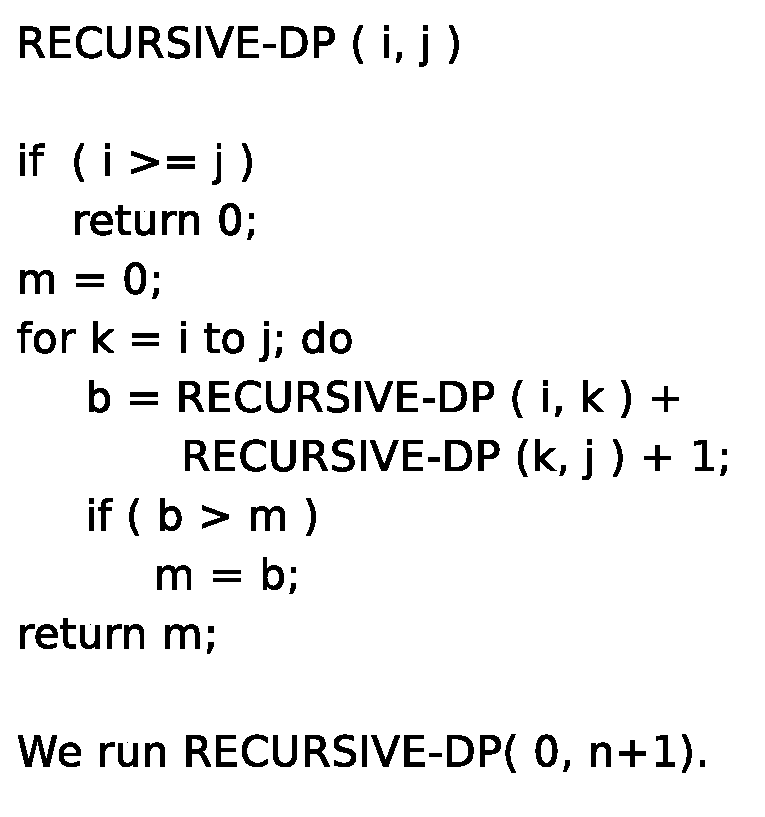
\includegraphics[width=1.0\textwidth]{L7-intervalschedulingdpalgo.eps}%
%      \end{minipage}%
%  \quad
%      \begin{minipage}{0.30\textwidth}
%       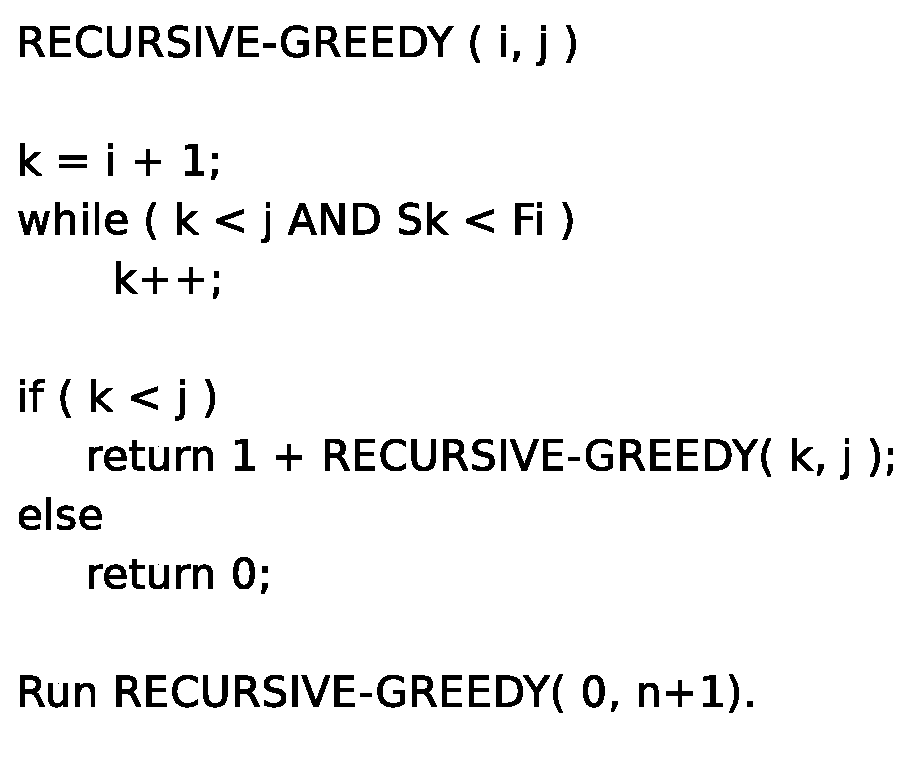
\includegraphics[width=1.0\textwidth]{L7-intervalschedulinggreedyalgo.eps}%
%      \end{minipage}%
%  \quad
%       \begin{minipage}{0.25\textwidth}
%       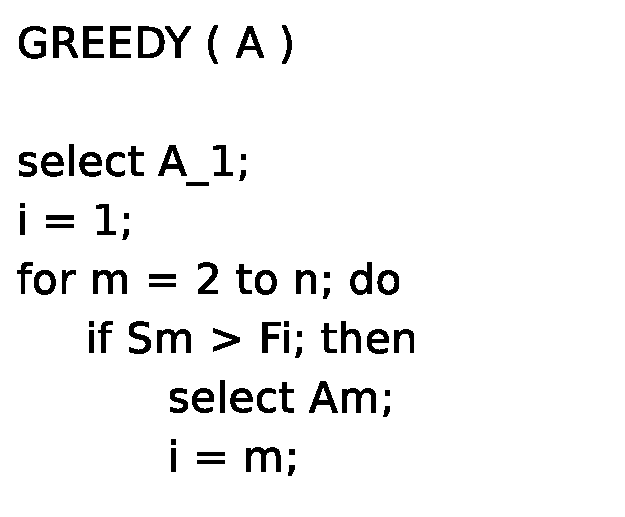
\includegraphics[width=1.0\textwidth]{L7-intervalschedulinggreedyalgo2.eps}%
%      \end{minipage}%
% 
%  \end{figure}

\title{CS711008Z  Algorithm Design and Analysis }
\subtitle{ Lecture 12. Randomized algorithm: a brief introduction
%\footnote{The slides were made based on Chapter 13 of Algorithm design, Randomized Algorithm by R. Motwani and P. Raghavan. } 
}
\author{Dongbo Bu } 
\institute{ {\small Institute of Computing Technology \\ 
Chinese Academy of Sciences, Beijing, China}}

\date{}

\begin{document}
%\begin{CJK}{UTF8}{cyberbit}

\frame{\titlepage}

\frame{
\frametitle{Outline}
\begin{itemize}
\item Introduction and nine categories proposed by R. Karp; 
\item The first example: {\sc GlobalMinCut} problem; 
\item Randomized algorithm in protocol design for distributed system; 
\item Randomization in approximation algorithm: LP+Random Rounding; 
\item Randomization coupled with divide-and-conquorer; 
\item Hashing
\end{itemize}

\textcolor{red}{Why randomized algorithm? Simplicity and speed. For many applications, a randomized algorithm is the simplest algorithm available, the fastest, or both.}
}

\frame{
\begin{block}{}
 A brief introduction
\end{block}
}

\frame{
\frametitle{ How to deal with hard problems? Trade-off ``quality'' and ``time''}

We have a couple of options: 
\begin{footnotesize}
 \begin{enumerate}
 \item Give up \textcolor{red}{polynomial-time} restriction: hope that our algorithms run fast on the practical instances. (e.g. branch-and-bound, branch-and-cut, and branch-and-pricing algorithms are used to solve a TSP instance with  over  24978 Swedish Cities. See http://www.tsp.gatech.edu/history/pictorial/sw24978.html)
 \item Give up \textcolor{red}{optimum} restriction: from ``optimal'' solution to ``nearly optimal'' solution in the hope that ``nearly optimal'' is easy to find. e.g., approximation algorithm (with theoretical guarantee), heuristics, local search (without theoretical guarantee); 
 \item Give up \textcolor{red}{deterministic} restriction: the expectation of running time of a randomized algorithm might be polynomial; 
 \item Give up \textcolor{red}{worst-case} restriction: algorithm might be fast on special and limited cases; 
 \end{enumerate}
\end{footnotesize}
} 



\frame{
\frametitle{ Deterministic  algorithm } 

 \begin{figure}
        \includegraphics[width=4in]{L12-deterministicalgo.eps}
\end{figure}

\begin{itemize}
\item
Goal: To prove that the algorithm solves the problem correctly (always) and quickly (typically, the  number of steps should be polynomial in the size of the input) 
\end{itemize}

(Excerpted from slides by P. Raghavan)

} 

\frame{
\frametitle{ Randomized  algorithm } 

 \begin{figure}
        \includegraphics[width=4in]{L12-randomizedalgo.eps}
\end{figure}

\begin{itemize}
\item
In addition to  input,  algorithm takes a source of random numbers and makes random 
choices during execution. 
\item 
Behavior can vary even on a fixed input 
\end{itemize}

} 


\frame{
\frametitle{Two views of randomness in the context of computation}
\begin{enumerate}
 \item The world is random: our algorithm is a deterministic algorithm that confront randomly generated input, and we can study the behavior of an algorithm on an ``average'' input rather than the worst-case input. 
 \item The algorithm is random: the world provides the same worst-case input as always; however, we allow our algorithm to make random decisions during execution.  
\end{enumerate}
   \begin{figure}
        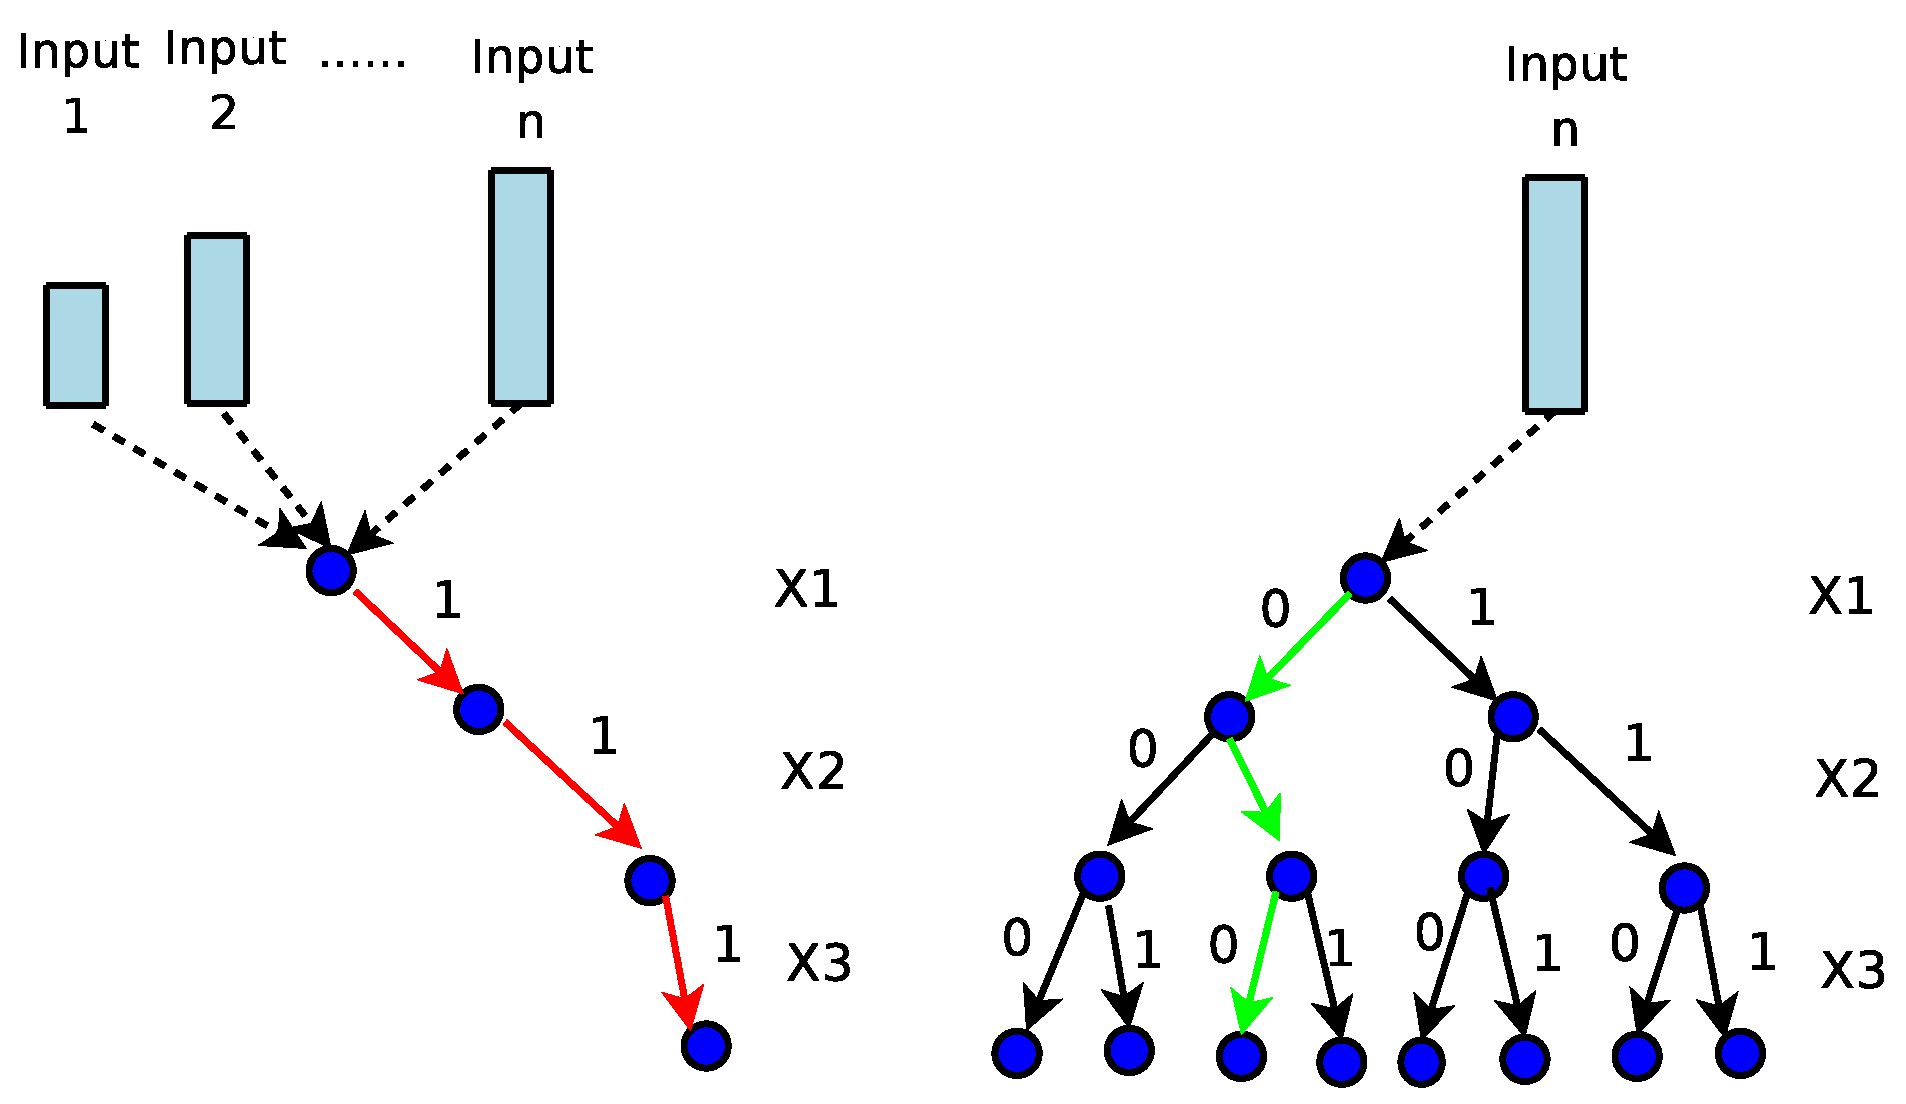
\includegraphics[width=2.8in]{L12-randomizedworldandalgo.eps}
   \end{figure}
} 

\frame{
\frametitle{Two types of randomzied algorithms}
\begin{enumerate}
 \item Las Vegas: always correct. Analyze its expected  running-time. 
 \item Monte Carlo: correctness depends on the random choice. Analyze its error probability. 
\end{enumerate}
Note:  still for worst-case input. ($\max_{Instance} \text{expected time}$, or $\max_{Instance} \Pr[ error ] $ );
}

\frame{
\begin{block}{}
Paradigms for randomized algorithms 
\end{block}
}

\frame[allowframebreaks]{
\frametitle{ Paradigms for randomized algorithm (by R. Karp) }
A handful of general principles lies at the heart of almost all randomized algorithms, despite the multitude of areas in which they find application. 
\begin{enumerate}
 \item Foiling an adversary: The classical adversary argument for a deterministic algorithm establishesa lower bound on the running time by constructing an input on which the algo fares poorly. While the adversary may be able to construct an input to foil one deterministic algo, it is difficult to devise a single input that is likely to defeat a randomized algo. (online algo, efficient proof verification)
 \item Random sampling: a random sample from a population is representative of the whole population; 
 \item Abundance of witnesses: To find a witness of a property of an input (say, ``$x$ is prime''). If the witness lies at a search space that is too large to search exhaustively, it suffices to randomly choose an element if the space contains a large number of witnesses. 
 \item Fingerprinting and hashing: to represent a long string by a short fingerprint using a random mapping. If two fingerprints are identical, the two strings are likely to be identical. 
 \item Random re-ordering input: After the re-ordering step, the input is unlikely to be in one of the orderings that is pathological for the naive algorithm; 
 \item Rapidly mixing Markov chains: To count the number of combinatorial objects, we can randomly sample an appropriately defined population, which in turn relies on the information of the number. Solution: defining a Markov chain on the elements, and  showing a short random walk is likely to sample the population uniformly. 
 \item Probabilistic methods and existence proofs: To establish that an object with cetain property exists by arguing that a randomly chosen object has the property with positive probability. 

\item Load balancing: To spread load evenly among the resources in a paralell or distributed environment,  where resource utilization decisions have to be made locally without reference to the global impact of these decisions. To reduce the amount of explicit communication or synchronization. 
 
\item Isolation and symmetry breaking: In parallel environment, it is usually important to require a set of processors to find the same solution (consensus): choosing a random ordering on the feasible solutions, and tehn requiring the processors to find the solution with the lowest rank. 
 
\end{enumerate}
}


\frame{
\begin{block}{}
 The first example: {\sc GlobalMinCut} problem 
\end{block}
}

\frame{
\frametitle{Graph algorithm:  {\sc GlobalMinCut} problem }
\begin{block}
{\bf INPUT: } A graph $G=<V,E>$\\

{\bf OUTPUT: } a cut $c=<A,B>$ such that the size of $c$ is minimized. Here, $A,B$ are non-empty vertex sets and $V=A\cup B$.\\
\end{block}

  \begin{figure}
        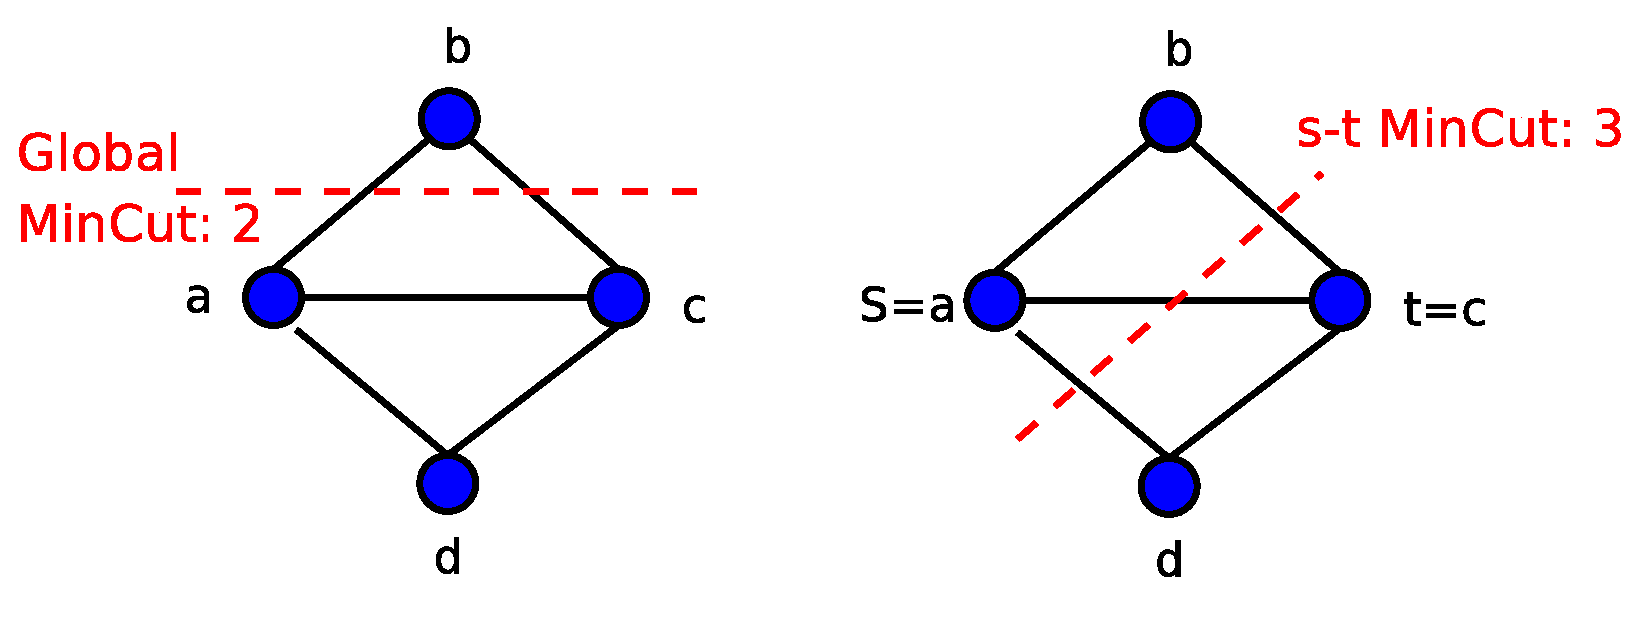
\includegraphics[width=3in]{L12-mincutexample.eps}
   \end{figure}

Note: The difference from the $s-t$ $cut$ problem, where two vertex $s$ and $t$ are given, and we restrict the cut: $s\in A$, and $t\in B$. 

}

\frame{
\frametitle{ A deterministic trial}
\begin{itemize}
 \item 
Basic idea: Transfering undirected graph $G$ to a directed graph $G'$ by replacing an edge $e=(u,v)$ with $e'=(u,v)$ and $e''=(v,u)$, each of capacity $1$. Let $s$ be an arbitrary node. For $t=2$ to $n$, call maximum-flow algorithm to calculate the minimum $s-t$ cut, and report the minimal one. 

\item 
Intuition: If $(A,B)$ is a minimum $s-t$ cut in $G'$, $(A,B)$ is also a minimum cut among all those that separates $s$ from $t$. We need a cut to seperate $s$ from something. 

\item 
Time-complexity: $O(n^4)$. 
\item 
Note: Gloabl minimum cut can be found as efficiently as $s-t$ cut by techniques that didn't requires augmentation-path or a notion of flow. 
\end{itemize}
} 


\frame{
\frametitle{ Randomized algorithm (D. Karger, '92) }

Advantage: qualitatively simpler than all previous algorithms. 

\begin{figure}
        \includegraphics[width=3.5in]{L12-Kargeralgoandexample.eps}
\end{figure}
   
\begin{itemize}
 \item 
Intuition: contracting an edge. When randomly selecting an edge, the probability to select an edge $e$ in the global min-cut is very small.
\item 
Multi-graph: multiple parallel edges between a pair of points $u$ and $v$. 
\end{itemize}
}

\frame{
\frametitle{ A Las Vegas algorithm for {\sc GlobalMinCut} problem} 

  \begin{figure}
        \includegraphics[width=4in]{L12-Kargeralgoexecution.eps}
   \end{figure}
}

\frame[allowframebreaks]{
\frametitle{Analysis}
\begin{Theorem}
The contraction algorithm returns a global min-cut with probabilty at least $\frac{1}{ C_n^2 }$.  
\end{Theorem}
Note: a bit counter-intuitive since there are exponentially many possible cuts of $G$, and thus the probabilty seems to be exponentially small. \\

Proof:  \\
  \begin{itemize}
   \item Suppose $(A,B)$ is a global min-cut with $k$ edges. We want a lower bound of the probability that Contraction algo returns $(A,B)$. 
   \item Complement: failure due to an edge $e=(u,v)$, $u\in A$, $v\in B$ is selected for contracting; 
   \item Let $F_i$ be the event that an edge $e$ in the cut is selected at the $i$-th iteration. We have: 
   \item (The $1$-st iteration) $Pr[ F_1 ] = \frac{k}{|E|} \leq \frac{k}{(1/2) kn} = \frac{2}{n}$. \\
   (Reason: Each node $v$ has a degree at least $k$. Otherwise, the cut $(v,V-v)$ has a size less than $k$. Thus, the edge number is at least $(1/2)kn$.)
   \item (The $j$-th iteration) $Pr[ F_j | \overline{F_{j-1}} ... \overline{F_{1}} ] \leq \frac{2}{n-j}$. \\
   (Reason: same argument to $G'$, where only $n-j$ supernodes are left.)
 \end{itemize} 

   \begin{eqnarray} 
     &&Pr[  \overline{F_{n-2}}\cap ... \cap \overline{F_{1}} ] \\
     &=& Pr[ \overline{F_{1}} ] Pr[ \overline{F_{2}} | \overline{F_{1}} ] ... Pr[ \overline{F_{n-2}} | \overline{F_{n-3}}\cap ... \cap \overline{F_{1}} ]\\
     &\geq& (1-\frac{2}{n})(1-\frac{2}{n-1})...(1-\frac{2}{3}) \\
     &=&\frac{n-2}{n} \frac{n-3}{n-1} \frac{n-4}{n-2}...\frac{1}{3}  \\
     &=&\frac{2}{n(n-1)} 
 \end{eqnarray}
}

\frame{
\frametitle{Further reduce failure probability via repeating}
Basic idea: running Contraction algo $r$ times will increase the probabilty to find a global min-cut. 

\begin{itemize}
 \item $r= C_n^2$: $Pr( FAILURE ) \leq (1-\frac{1}{C_n^2})^{C_n^2} \leq \frac{1}{e}$.
 \item $r= C_n^2 \ln n$: $Pr( FAILURE ) \leq (1-\frac{1}{C_n^2})^{ C_n^2\ln n } \leq \frac{1}{e^{\ln n}} = \tfrac{1}{n}$.
\end{itemize}

Time complexity: $O( r m)$ (Contraction algo costs $O(m)$ time.)
}

\frame{
\frametitle{ Extension: the number of GloablMinCut }
\begin{itemize}
\item 
Question: what is the maximum number of global min-cuts an undirected graph $G$ can have? 
\item 
Not obvious. Consider a directed graph as follows:   
$s$ together with any subset of $v_1,...,v_n$ constitutes a minimum $s-t$ cut. ( $2^n$ cuts in total.)
\end{itemize} 

\begin{figure}
        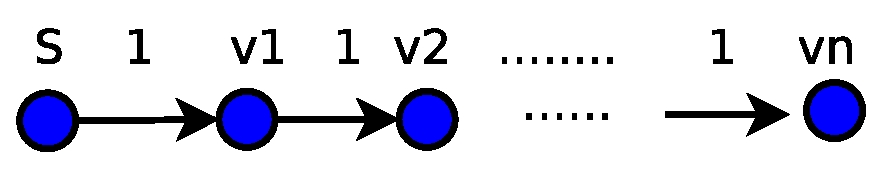
\includegraphics[width=2in]{L12-mincutnumber.eps}
   \end{figure}
} 

\frame{
\frametitle{ Extension: the number of GloablMinCut cont'd }

\begin{Theorem}
 An undirected graph $G$ on $n$ nodes has at most $ C_n^2$ global min-cuts. 
\end{Theorem}
Proof: \\
 \begin{itemize}
  \item Suppose there are $r$ global min-cut $c_1,...,c_r$; 
  \item Let $C_i$ denote the event that $c_i$ is reported, and $C$ denote the success of Contraction algo;
  \item For each $i$, we have $Pr[ C_i ] \geq \frac{1}{C_n^2}$.
  \item Thus $Pr[ C ] = Pr[ C_1 \cup ... \cup C_r ] $\textcolor{red}{=}$ \sum_i Pr[ C_i ] \geq r \frac{1}{C_n^2}$. (Note: $=$ since all $C_i$ are disjoint. )
  \item We get $r \leq C_n^2 $. ($ r \frac{1}{C_n^2} \leq 1$.)
 \end{itemize}
}

\frame{
\begin{block}{}
 Randomization in distributed computing 
\end{block}
}

\frame{
\frametitle{Protocol design:  {\sc ContentionResolution} }
\begin{block}{}
\begin{small}
{\bf INPUT:} \\ Suppose we have $n$ nodes $M_1,..., M_n$, each competing for access to a single shared database. The database can be accessed by at most one node in a single time slice; if two or more nodes attempt to access it simultaneously, then all nodes are ``locked out'' for the duration of that slice. \\
{\bf GOAL: } \\ to design a protocol to divide up the time slices among the nodes in an equitable fashion. (suppose that the nodes cannot communicate with one another at all.) 
\end{small}
\end{block}

  \begin{figure}
        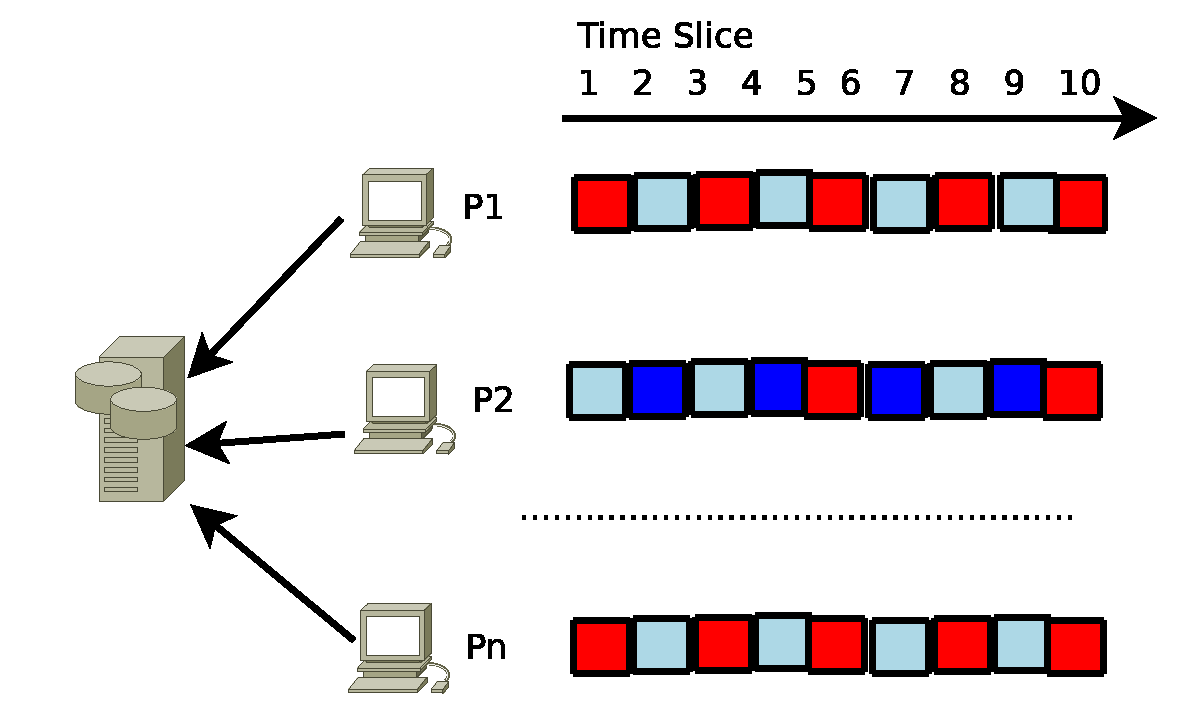
\includegraphics[width=1.8in]{L12-contentionprotocol1.eps}
   \end{figure}
}

\frame{
\frametitle{Protocol design:  {\sc ContentionResolution} }
\begin{itemize}
\item 
A randomized algorithm: 
{\it Each node will attempt to access the database at each slice with probability $p$, independently of the decisions of others.}
\item 
Intuition: each node randomizes its behavior. 
\item 
Symmetry-breaking strategy: If all nodes operated in lockstep, repeatedly trying to access the database at the same time, there'd be no progress; but by randomizing, they ``smooth out'' the contention. 
\end{itemize} 

\begin{figure}
        \includegraphics[width=2.in]{L12-contentionprotocol2.eps}
\end{figure}
}

\frame{
\frametitle{Analysis of the protocol}
{\bf Waiting for a particular node to succeed. }
\begin{Theorem}
After $\Theta(n)$ time slices, that probability that $M_i$ has not yet succeeded is less than a constant;  and after $\Theta(n\ln n)$ time slices, the probability drops to a quite small quantity. 
\end{Theorem}
} 
\frame{ 
\begin{small}
\begin{Proof}
\begin{itemize}
   \item Let $A(i,t)$ denote the event that $M_i$ attempts to access DB at time $t$, and $S(i,t)$ denote the success of the access. 
   \item We have:  $Pr[ S(i,t) ] = Pr[ A(i,t)] \times \prod_{j\neq i} Pr[ \overline{ A(j,t) } ] = p(1-p)^{n-1}$ 
   \item By setting the derivative to $0$, we get $p=\frac{1}{n}$. And the maximum of $Pr[ S(i,t) ]$ is achieved: $Pr[ S(i,t) ]=\frac{1}{n}(1-\frac{1}{n})^{n-1}$.
   \item $ \frac{1}{en} \leq Pr[ S(i,t) ] \leq \frac{1}{2n}$. (Reason: As $n$ increases from 2, $(1-\frac{1}{n})^n$ coverges monotonically from $\frac{1}{4}$ to $\frac{1}{e}$, and $(1-\frac{1}{n})^{n-1}$ coverges monotonically from $\frac{1}{2}$ to $\frac{1}{e}$. ) \\
   \item Let $F(i,t)$ denote the ``failure event'' that $P_i$ does not succeed in any of the slices 1 through $t$; 
   \item $Pr[ F(i,t) ] = \prod_{r=1}^t Pr[ \overline{S(i,r)} ]= ( 1 - \frac{1}{n}(1-\frac{1}{n})^{n-1} )^t$. 
   \item A simpler estimation: $Pr[ F(i,t) ] = \prod_{r=1}^t Pr[  \overline{S(i,r)} ] \leq  ( 1 - \frac{1}{en} )^t$. 
   \item $Pr[ F(i,t) ]  \leq  ( 1 - \frac{1}{en} )^t \leq \frac{1}{e}$ when setting $t$ to $en$.
   \item $Pr[ F(i,t) ]  \leq  ( 1 - \frac{1}{en} )^t \leq (\frac{1}{e})^{c \ln n } = n^{-c}$ when setting $t$ to $c e n \ln n  $.
  \end{itemize}
\end{Proof}
\end{small}
}

\frame{
\frametitle{Analysis of the protocol}
{\bf Waiting for all  nodes to succeed. }
\begin{Theorem}
With probability at least $1-n^{-1}$, all nodes succeed in accessing the DB at least once within $t=2en \ln n$ time slices. 
\end{Theorem}
\begin{Proof}
\begin{itemize}
   \item Let $F(t)$ denotes the event that some nodes have not yet accessed DB after $t$ time slices; 
   \item $Pr[ F(t) ] = Pr[ \bigcup_{i=1}^n F(i,t) ] \leq \sum_{i=1}^n Pr[F(i,t) ] $  
   \item $Pr[ F(t) ] \leq n \times n^{-c}$ after $t=c en\ln n$ time slices. 
   \item In particular, $Pr[ F(t) ] \leq \frac{1}{n}$ after $t=2 en\ln n$ time slices. 
  \end{itemize}
\end{Proof}
}

\frame{
\frametitle{Protocol design in distributed system: {\sc LoadBalance} }
\begin{block}{}
 {\bf INPUT: } $n$ processors $P_1,...,P_n$, and $m$ jobs arrive in a stream and need to be processed immediately; \\
 {\bf GOAL: } to design a protocol to distribute jobs among processors evenly. (Assuming no central controller again.)
\end{block}

Randomized algorithm: {\it assign each job to one of the processors uniformaly at random.}
}

\frame[allowframebreaks]{
\frametitle{Analysis: how well does this simple algo work?}
\begin{Theorem}
(A simple case: $m=n$) With probability at least $1-n^-1$, there is no processor that was assigned with over $e\gamma(n) = \Theta( \frac{\log n } { \log \log n} )$ jobs.  
\end{Theorem}
\begin{footnotesize}
\begin{Proof}
\begin{itemize}
\item Let $X_i$ denote the number of jobs assigned to $P_i$. Define an index random variable $Y_{ij}$ as follows: $Y_{ij}=1$ when job $j$ is assigned to $P_i$, and $0$ otherwise. 
\item We have:  $X_i = \sum\nolimits_{j=1}^n Y_{ij}$. 
\item Then, 
\begin{eqnarray}
E(X_i) &=& E( \sum\nolimits_{j=1}^n Y_{ij} ) \nonumber \\
       &=& \sum\nolimits_{j=1}^n E( Y_{ij} ) \nonumber \\
       &=& \sum\nolimits_{j=1}^n Pr( Y_{ij} = 1 ) \nonumber \\
       &=& n  \times \tfrac{1}{n} = 1 \nonumber 
\end{eqnarray}

\item Thus $Pr[ X_i > c ] < \frac{e^{c-1}}{c^c}$   (by Chernoff bound.)
\item Suppose we have a $c$ such that $Pr[ X_i > c ] < \frac{e^{c-1}}{c^c} \leq \frac{1}{n^2}$, then $Pr[ \exists i, X_i > c  ] \leq n\times \frac{1}{n^2} = \frac{1}{n}$. 
\end{itemize}
\end{Proof}

\end{footnotesize}
}

\frame{
\frametitle{The remaining difficulty: how to choose a $c$? }
\begin{itemize}
 \item 
Let $\gamma(n)$ be the solution to $x^x=n$. The estimation of $\gamma(n)$ can be given as follows: \\
\item Taking logarithm of $x^x=n$ gives: $x \ln x = \ln n$. 
\item Taking logarithm again: $\ln x + \ln\ln x = \ln \ln n$. 
\item We have: $ \ln x \leq \ln \ln n = \log x +  \ln \ln x \leq  2\ln x$ (by $log(log(x)) \leq log(x)$ Dividing the equation: $x \ln x = \ln n$ (by $ln ln (n) \geq 0$ when $n\geq e^e$) , we get: 
\item $ \frac{1}{2} x \leq \frac{\ln n}{\ln \ln n} \leq x = \gamma({n})$. 
\item Setting $c=e\gamma(n)$, we have: $Pr[ X_i > c ] < \frac{e^{c-1}}{c^c} < (\frac{e}{c})^c =(\frac{1}{\gamma(n)})^{e\gamma(n)}<(\frac{1}{\gamma(n)})^{2\gamma(n)} = \frac{1}{n^2}$. 
\end{itemize}
} 

\frame{
\frametitle{$\gamma(n)$: the solution to $x^x=n$ }


  \begin{figure}
        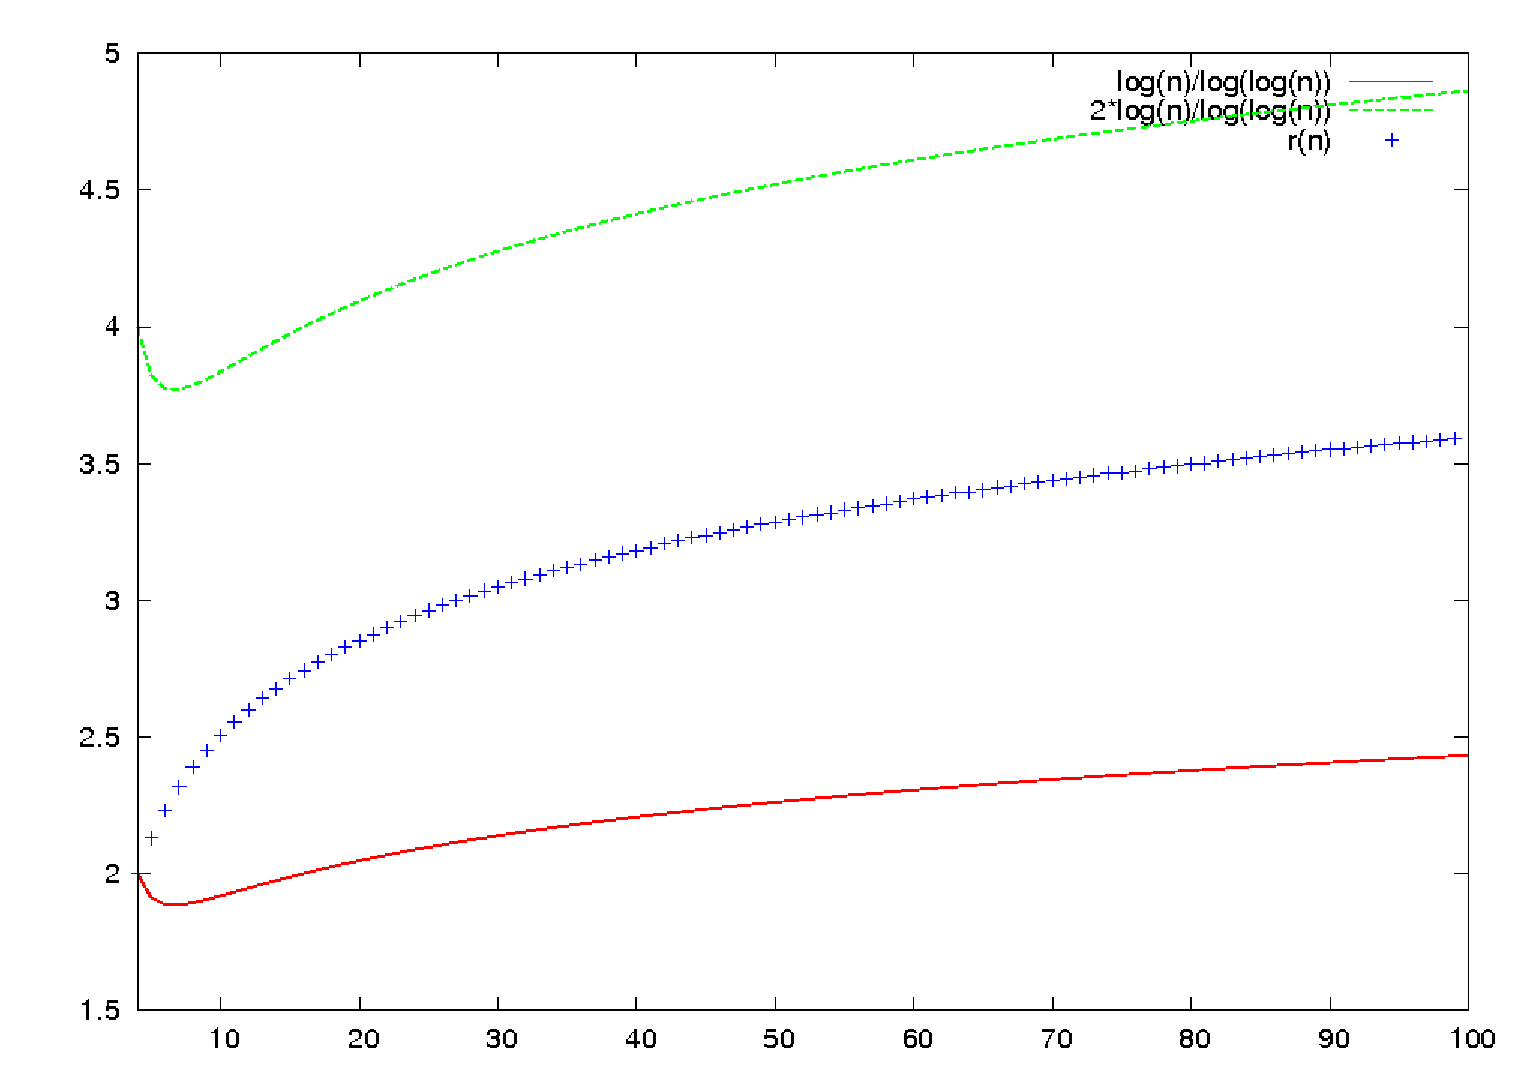
\includegraphics[width=3in]{L12-GammaN.eps}
   \end{figure}
}

\frame{
\frametitle{ More jobs } 
\begin{itemize}
 \item 
More jobs: ($m=6 n \ln n$) The expected jobs number is: $\mu = 6 \ln n$. We have: 
\item 
$Pr[ X_i > 2\mu ] < (\frac{e}{4})^{6\ln n} < (\frac{1}{e^2})^{\ln n} = \frac{1}{n^2}$. (by $(\frac{e}{4})^6 < \frac{1}{e^2}$.) 

\end{itemize}
} 

\frame{
\begin{block}{}
 Bounding the sum of independent random variables 
\end{block}
}

\frame{
\frametitle{ Bound 1: Markov inequality}
\begin{itemize}
 \item Suppose $X$ is a non-negative random variable with mean $u=E(X)$. 
 \item We have: 
 $\Pr [  X  \geq  t ] \leq \frac{E(X)}{t}$. 
 \end{itemize}
 
  \begin{figure}
        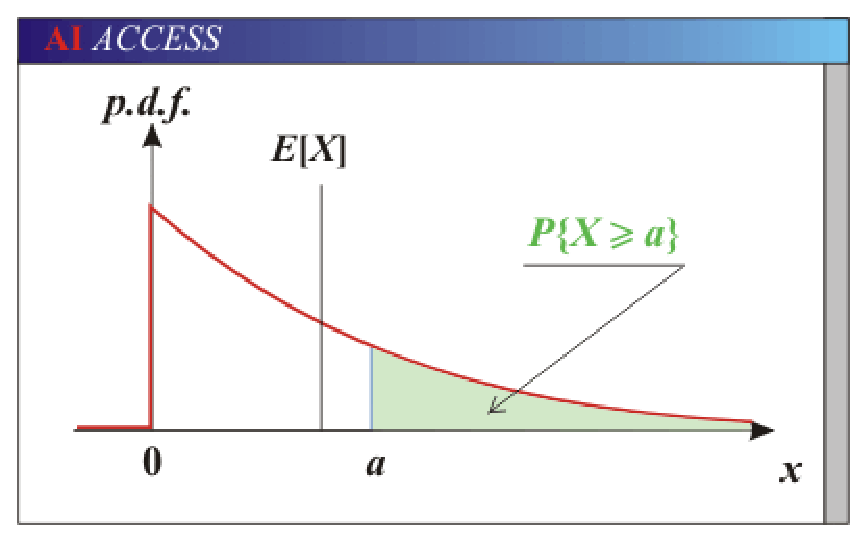
\includegraphics[width=2in]{L12-markov-inequality.eps}
   \end{figure}
 
}

\frame{
\frametitle{ Bound 2: Chebyshev inequality}
\begin{itemize}
 \item Suppose $X$ is a random variable with mean $u=E(X)$, and variance $\sigma^2 = Var(X)$. 
 \item We have: 
 $\Pr [ | X - u | \geq  k \sigma  ] \leq \frac{1}{k^2}$. 
 \end{itemize}
 
   Note: the non-negative requirement is removed, but need the information of variance. 
}

\frame[allowframebreaks]{
\frametitle{Bound 3: Chernoff bound (upper bound) }
\begin{Theorem} (Upper bound) 
 Let $X=X_1+X_2+...+X_n$, where $X_i$ is $0/1$ variable that takes $1$ with probability $p_i$. Define $\mu=E(X)=\sum_i p_i$. For any $\delta > 0$, we have: $Pr[ X > (1+\delta)\mu ] < (\frac{e^\delta}{(1+\delta)^{(1+\delta)} })^\mu$. 
\end{Theorem}
(Intuition: the flucuations of $X_i$ are likely to be ``cancelled out'' as $n$ increases.)
\begin{Proof}  
 \begin{itemize}
 \item Step 1: $Pr[ X > (1+\delta)\mu ] = Pr[ tX > t(1+\delta)\mu ] = Pr[ e^{t X} > e^{t (1+\delta)\mu} ] \leq \frac{E(e^{t X})}{ e^{t (1+\delta)\mu} } $ for any $t>0$. 
 (Applying Markov inequality on $e^{tX}$)
 \item Step 2: $E(e^{tX}) = E(e^{tX_1+...+tX_n}) = E( e^{tX_1}... e^{tX_n} ) $  (by independence of $X_i$.)
 \item Step 3:  $E(e^{tX_i})= e^t p_i + 1 (1-p_i) = 1 + p_i(e^t -1) \leq e^{p_i} ( e^t-1) $ (by $1+x\leq e^x$, for $x>0$.)
 \item Thus we have: $Pr[ X > (1+\delta)\mu ] \leq \frac{E(e^{t X})}{ e^{t (1+\delta)\mu} }\leq  \frac{\prod_i e^{p_i (e^t-1)} }{ e^{t (1+\delta)\mu} } = \frac{ e^{\mu (e^t-1)} }{ e^{t (1+\delta)\mu} }$.
 \item Step 4: Setting $t=\ln(1+\delta)$. 
 \end{itemize}
\end{Proof}
} 

\frame[allowframebreaks]{
\frametitle{Bound 3: Chernoff bound (lower bound) }

\begin{Theorem}
(Lower bound) 
 Let $X=X_1+X_2+...+X_n$, where $X_i$ is $0/1$ variable that takes $1$ with probability $p_i$. Define $\mu=E(X)=\sum_i p_i$. For any $\delta > 0$, we have: $Pr[ X <  (1-\delta)\mu ] < e^{ - \frac{1}{2} \mu \delta^2}$. 
\end{Theorem}
}


\frame{
\frametitle{ Comparison of Markov inequality and Chernoff bound } 

 \begin{figure}
        \includegraphics[width=3in]{L12-comparing-bounds.eps}
   \end{figure}

Trial: The number of heads in 100 tosses of a coin. $Pr[ head ] = 0.75 $. 
Lines: The real probability (in red); Markov bound (in blue); Chernoff bound (in green). 
} 



\frame{
\begin{block}{}
LP+Random rounding paradigm: {\sc MaxSAT} problem 
\end{block}
}

\frame{
\frametitle{ A randomized approximation algorithm for {\sc Max3Sat} }
\begin{block}{}
 {\bf INPUT: } \\ Given a set of clauses $C_1,...,C_k$, each of length 3, over a set of boolean variables $X=\{x_1,...,x_n\}$; \\
 {\bf OUTPUT: } \\ to find an assignment to maximize the number of satisfied clauses; 
\end{block}
e.g. \\
$C1: $ $x_1 \vee \neg x_2 \vee x_3$ \\
$C2: $ $\neg x_1 \vee \neg x_2 \vee x_4$ \\
$C3: $ $\neg x_3 \vee \neg x_4 \vee x_5$ \\
$C4: $ $\neg x_2 \vee \neg x_4 \vee x_7$\\
} 


\frame{
\frametitle{ Algo1 }

Algo1 (remarkably simple):
\begin{algorithmic}[1]
\STATE  set each variable $x_i$ to $1$ with probability $\frac{1}{2}$. 
\end{algorithmic}
} 

\frame{
\frametitle{ Algo1 is good }
\begin{Theorem}
 The expected number of clauses satisfied by Algo1 is within an approximation factor $\tfrac{7}{8}$ of optimal. 
\end{Theorem}
\begin{Proof}
 \begin{itemize}
  \item Let $X$ be the number of satisifed clauses. $X_i$ is an index variable such that $X_i=1$ if $C_i$ was satisfied, and $X_i=0$ otherwise. 
 \item $X=X_1+...+X_k$
 \item $E(X)=E(X_1+...+X_k) = E(X_1)+...+E(X_k) = \frac{7}{8}k$ ($E(X_i) = \frac{7}{8}$)
 \item and we have a lower bound: $OPT \leq k$. 
 \item Thus, $E(X) \geq \frac{7}{8} OPT$. 
 \end{itemize}
\end{Proof}
} 


\frame{
\frametitle{ Extensions}

Probability method: 
\begin{corollary}
 There exists at least an assignment to satisfy at least $\tfrac{7}{8}k$ clauses.
\end{corollary}
(Intuition: the expectation is over $\tfrac{7}{8}k$ clauses. Just an existence proof. )

} 

\frame{
\frametitle{ Extensions}

Probability method again: 
\begin{corollary}
 All 3SAT instance with at most $7$ clauses are satisfied. 
\end{corollary}
(Intuition: The unsatisfied clause number is $\tfrac{1}{8} k= \frac{7}{8} < 1 $. )

} 

\frame{
\frametitle{ Algo 2 }

\begin{itemize}
 \item 
Question: how to find an assignment to satisfy at least $\tfrac{7}{8}k$ clauses? 
\item
Algo 2:  

\begin{algorithmic}[1]
\STATE  repeat Algo1 until at least $\tfrac{7}{8}k$ clauses are satisfied. 
\end{algorithmic}

\end{itemize}
}

\frame[allowframebreaks]{
\frametitle{ Find a good assignment: analysis }
\begin{Theorem}
 The expected running time of Algo2 is polynomial. In particular, the expected number of $repetition$ is less than $8k$.
\end{Theorem}
\begin{Proof}
 \begin{itemize}
  \item Let $p$ be the probability that at least $\tfrac{7}{8}$ clauses are satisfied; 
  \item It suffices to prove that $\tfrac{1}{p} \leq 8k$. (Reason: the expected waiting time of an event with probability $p$ is $\tfrac{1}{p}$.)
  \item Let $p_j$ be the probability that EXACTLY $j$ clauses are satisfied. We have: 
\begin{enumerate}
 \item  $p=\sum_{j \geq \tfrac{7}{8} k} p_j$, \\
\item $p +  \sum_{j < \tfrac{7}{8} k} p_j = 1$; \\
\item  $E(X)=\tfrac{7}{8}k = \sum_{j=1}^k j p_j = \sum_{j \geq \tfrac{7}{8} k} j p_j  + \sum_{j < \tfrac{7}{8} k} j p_j$.
\end{enumerate}
\end{itemize}
\begin{itemize}
  \item Thus, $ \tfrac{7}{8}k \leq  \sum_{j \geq \tfrac{7}{8} k} k p_j  + \sum_{j < \tfrac{7}{8} k} k' p_j = k p + k'(1-p) \leq k' + k p$. ($k'$ is the max number such that $k'<\tfrac{7}{8}k$.)
  \item Thus, $k p \geq \tfrac{7}{8}k - k'$, and $ p \geq \tfrac{1}{8k}$. (since $\tfrac{7}{8}k - k' \geq \tfrac{1}{8}$.)
 \end{itemize}
\end{Proof}
}

\frame{
	\begin{block}{}
	Algo3: ``LP+Random Rounding'' strategy
	\end{block} 
}

\frame{
\frametitle{ ILP formulation }

$C1: $ $x_1 \vee \neg x_2 \vee x_3$  \\
$C2: $ $\neg x_1 \vee \neg x_2 \vee x_4$  \\
$C3: $ $\neg x_3 \vee \neg x_4 \vee x_5$  \\
$C4: $ $\neg x_2 \vee \neg x_4 \vee x_7$ \\

ILP: 
\[
\begin{array}{rrrrrrrrl}
 \max &z=& z_1 + z_2 + ... z_k  \\
 s.t. && x_1 + (1-x_2) + x_3  &\geq& z_1  \\ 
      && (1-x_1) + (1-x_2) + x_4 &\geq& z_2 \\
&& (1-x_3) + (1-x_4) + x_5 &\geq& z_3 \\
&& x_i &=& 0/1 \\
      && z_j &=& 0/1 \\
\end{array} \nonumber
\]
} 


\frame{
\frametitle{ Relax ILP to LP }

LP: 
\[
\begin{array}{rrrrrrrrl}
 \max &z=& z_1 + z_2 + ... z_k&  \\
 s.t. && x_1 + (1-x_2) + x_3  &\geq& z_1  \\ 
      && (1-x_1) + (1-x_2) + x_4 &\geq& z_2 \\
&& (1-x_3) + (1-x_4) + x_5 &\geq& z_3 \\
& & ...... & & \\
      && x_i &\leq& 1 \\
      && z_j &\leq& 1 \\
\end{array} \nonumber
\]

} 

\frame{
\frametitle{ LP + Random Rounding }

Algo3: 

\begin{algorithmic}[1]
\STATE  Let $x^*,z^*$ denote the optimal solution to LP. 
\STATE Randomly set variable $x_i=TRUE$ with probability $x_i^*$. 
\end{algorithmic}

} 


\frame{
\frametitle{ Performance }

\begin{Theorem}
 A clause $C_j$ is satisfied with a probability at least $( 1 - (1-\tfrac{1}{3})^3) z_j^*$. 
\end{Theorem}
\begin{Proof}
Suppose w.l.o.g $C_j = x_1 \vee x_2 \vee x_3$. We have: 
 
 \begin{eqnarray*}
 Pr( C_j \text{ is satisfied} ) &=&  1 - (1-x_1^*)(1-x_2^*)(1-x_3^*)  \nonumber\\ 
 &\geq& 1 - ( \tfrac{1}{3} ( (1-x_1^*)+(1-x_2^*)+(1-x_3^*) ) )^3  \quad\text{( by Fact 1.)} \nonumber\\
 &\geq& 1 - ( 1 - \tfrac{1}{3} z_j^*   )^3 \quad\text{( by Fact 2.)} \nonumber\\
 &\geq& (1 - ( 1 -  \tfrac{1}{3})^3)  z_j^* \quad\text{( by Fact 3.)} \nonumber\\
 \end{eqnarray*}
\end{Proof}

} 

\frame{
\frametitle{ Some facts  }

\begin{itemize} 
\item 
Fact 1: The opitmal solution satisfies: $x_1^* + x_2^* + x_3^* \geq z_j^*$. 
\item 
Fact 2: $(x_1x_2...x_n)^{\tfrac{1}{n}} \leq \tfrac{1}{n}(x_1+x_2+...+x_n) $\\
\item 
Fact 3: $f(x)=1 - ( 1 - \tfrac{1}{3} x   )^3$ is concave, and greater than $g(x)=(1-(1-\tfrac{1}{3})^{3}) x$ at the two ends of $[0,1]$. Thus, $f(x) \geq g(x)$ for any $x\in[0,1]$.
\end{itemize} 
  \begin{figure}
        \includegraphics[width=1.8in,angle=270]{L12-max3sattwocurves.eps}
 \end{figure}
} 

\frame{
%\frametitle{ LP + Random Rounding is good }
\begin{Theorem}
 (Goemans, W '94) Algo3  is a $(1-\tfrac{1}{e})$-approximation algorithm, where $(1-\tfrac{1}{e})=0.632$. 
\end{Theorem}
\begin{small}
\begin{Proof}
Let $X$ be the number of satisfied clauses. Let index variable $c_j$ be 1 when clause $C_j$ is satisfied, and 0 otherwise. Thus, $X=c_1+c_2...+c_k$. 
\begin{eqnarray*}
E(X) &=&E(c1)+E(c_2)+...+E(c_k) \nonumber  \\ 
&=&\sum\nolimits_j Pr( C_j \text{ is satisfied} ) \quad \text{ (previous theorem)} \nonumber \\
&\geq& \sum\nolimits_j ( 1 - (1-\tfrac{1}{3})^3) z_j^* \nonumber  \\
&\geq& (1 - (1-\tfrac{1}{3})^3) \sum\nolimits_j z_j^* \nonumber \\
&=& (1 - (1-\tfrac{1}{3})^3) z_{LP}  \nonumber \\
&\geq& (1 - (1-\tfrac{1}{3})^3) OPT  \quad (\text{by } z_{LP} \geq z_{ILP} = OPT ) \nonumber \\ 
&\geq& (1 - \tfrac{1}{e} ) OPT  \quad (\text{by } (1-\tfrac{1}{n})^n \leq \tfrac{1}{e} ) \nonumber  
\end{eqnarray*} 
\end{Proof}
\end{small}
}

\frame{
\begin{block}{}
LP+Random rounding paradigm: {\sc VLSI Design} problem 
\end{block}
}


\frame[allowframebreaks]
{
\frametitle{Problem Statement}
\begin{itemize}
	\item A \emph{gate-array} is a two-dimensional $\sqrt{n} \times \sqrt{n}$ array of gates abutting each other.
	\item A \emph{net} is a set of gates to be connected by a wire. In our problem, the number of gates in a set is exactly 2.
	\item Assume that the wire for each net contains at most one $90^o$ turn, called ``one-bend'' route. Thus,
	in joining the two end-points of a net, the wire will either first traverse the horizontal dimension and then the vertical
	dimension, or the other way around. In particular, a net , which connects two gates in the same column or the same row, only has one choice.
	\item Let $w_S(b)$ denote teh number of wires that pass through \emph{boundary} $b$ in a solution $S$. Here, each of the four edges of a grid is called a \emph{boundary} $b$. 
\end{itemize}

The Problem is $\min_{S}\max_{b} w_S(b)$. (Intuition: not too many wires pass through any boundary.)

\begin{center}
 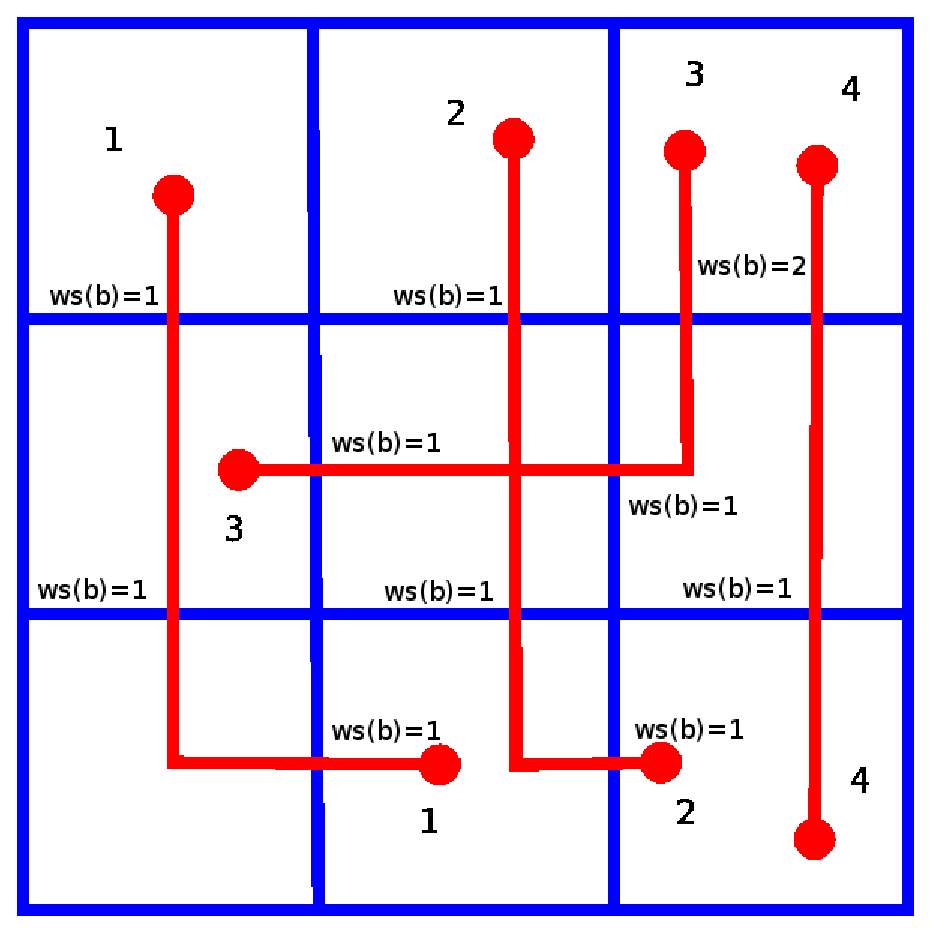
\includegraphics[width=0.5\textwidth]{L12-VLSI.eps}
 \end{center}
}

\frame[allowframebreaks]
{
\frametitle{Algorithm}
\begin{itemize}
 \item 

This problem can be cast as a $0-1$ linear program (because for each net, there is at most 2 choices.).
\item 
For each net $i$ from left end-point to the right end-point, we define 2 variables $x_{i0}$ and $x_{i1}$ to describe the direction of the wire:
\begin{eqnarray*}
	x_{i0} = 1, x_{i1} = 0 & \textrm{if net $i$ goes horizontally first}\\
	x_{i0} = 0, x_{i1} = 1 & \textrm{if net $i$ goes vertically first}
\end{eqnarray*}
\item
For each boundary $b$ in the array, let
\begin{eqnarray*}
	T_{b0} & = & \{i|\textrm{net $i$ passes through $b$ if $x_{i0}$ = 1}\}\\
	T_{b1} & = & \{i|\textrm{net $i$ passes through $b$ if $x_{i1}$ = 1}\}
\end{eqnarray*}
\end{itemize}

\begin{itemize}
 \item 
With these definitions, our integer program can be expressed as:
\begin{eqnarray*}
	\min w & & \\
	x_{i0} + x_{i1} &=& 1 \quad \forall i \\
	\sum_{i\in T_{b0}} x_{i0} + \sum_{i\in T_{b1}} x_{i1} & \le & w \quad \forall b \\
	x_{i0}, x_{i1} & \in & \{0, 1\}
\end{eqnarray*}
\item 
Let  ${OPT}$ be the objective value of the above $ILP$.
\item 
We solve instead the linear program relaxation of $ILP$ by replacing  $x_{i0}, x_{i1}  \in  \{0, 1\}$
to $x_{i0}, x_{i1} \in [0, 1]$ :
\begin{eqnarray*}
	\min w & & \\
	x_{i0} + x_{i1} &=& 1 \quad \forall i \\
	\sum_{i\in T_{b0}} x_{i0} + \sum_{i\in T_{b1}} x_{i1} & \le & w \quad \forall b \\
	x_{i0}, x_{i1} & \in & [0, 1]
\end{eqnarray*}
\end{itemize}
Let $\hat{x_{i0}}$ and $\hat{x_{i1}}$ be the solution, $\hat{w}$ be the objective value, of the above $LP$.
Obviously, $\hat{w} \le OPT$.

} 

\frame{
\frametitle{ LP +Random Rounding } 

\begin{itemize}
 \item 
Algo: \emph{Randomized Rounding } $\hat{x_{i0}}$ and $\hat{x_{i1}}$ to 0 and 1. \\
\item 
Indepently for each $i$, define 2 random variables, $\bar{x_{i0}}$ and $\bar{x_{i1}}$.
\begin{eqnarray*}
	Pr(\bar{x_{i0}} = 1, \bar{x_{i1}} = 0) & = & \hat{x_{i0}}\\
	Pr(\bar{x_{i1}} = 1, \bar{x_{i0}} = 0) & = & \hat{x_{i1}}
\end{eqnarray*}
\item Obviously, $E(\bar{x_{i0}}) = \hat{x_{i0}}$ and $E(\bar{x_{i1}}) = \hat{x_{i1}}$. 
\item Now we get a solution $S=\{\hat{x_{i0}}, \hat{x_{i1}}, i=1,2,...,n \}$ to the problem, how about its performance?
\end{itemize}
}

\frame[allowframebreaks]
{
\frametitle{Analysis}
\begin{block}{Theorem}
	Let $\epsilon$ be a real number such that $0 < \epsilon < 1$. Then with probability $1-\epsilon$, 
	the solution $S$ produced by randomized rounding satisfies
	$ w_S \le ( 1 + \Delta(\hat{w}, \epsilon/2n)) \hat{w} \le ( 1 + \Delta(OPT, \epsilon/2n)) OPT$.\\
	where $\Delta(\mu, \epsilon)$ is defined as : if let $\left[\frac{e^{\delta}}{(1+\delta)^{1+\delta}} \right] ^ {\mu} = \epsilon$,
	then $\delta = \Delta(\mu, \epsilon)$.
\end{block}


{\bf Proof}\\
\begin{itemize}
\item 
	The second inequality is obvious.
\item
	In order to prove the first inequality, we just need to prove that : for any boundary $b$,
	the probability that $w_S(b) > \hat{w} ( 1 + \Delta(\hat{w}, \epsilon/2n))$ is at most $\epsilon / 2n$. (Why?)
\item
	Consider a boundary $b$, $w_S(b) = \sum_{i\in T_{b0}} \bar{x_{i0}} + \sum_{i\in T_{b1}} \bar{x_{i1}}$ then
	$E(w_S(b)) = \sum_{i\in T_{b0}} E(\bar{x_{i0}}) + \sum_{i\in T_{b1}} E(\bar{x_{i1}}) =  
	\sum_{i\in T_{b0}} \hat{x_{i0}} + \sum_{i\in T_{b1}} \hat{x_{i1}} \le \hat{w}$
\item
	According to the Definition of $\Delta$ and Chenoff Bound, we have
	$Pr(w_S(b) > \hat{w}(1+\Delta(\hat{w}, \epsilon/2n))) \le \epsilon/2n$
	and the theorem follows.
\end{itemize}
}

\frame{
\begin{block}{}
 Randomized divide-and-conquorer
\end{block}
}

\frame[allowframebreaks]{
\frametitle{ Randomized divide-and-conquorer: {\sc Selection } problem }

\begin{block}{}
{\bf INPUT: } \\
Given a set of number $S=\{a_1,a_2,...,a_n\}$, and a number $k\leq n$;  \\
{\bf OUTPUT: } \\ 
the median in $S$, or the $k$-th smallest item. 
\end{block}

Note: known deterministic linear algorithms, say Blum '73 ($16n$ comparisons), and D. Zuick '95 ($2.95n$ comparisons). 

Randomized algorithm: 
 \begin{figure}
        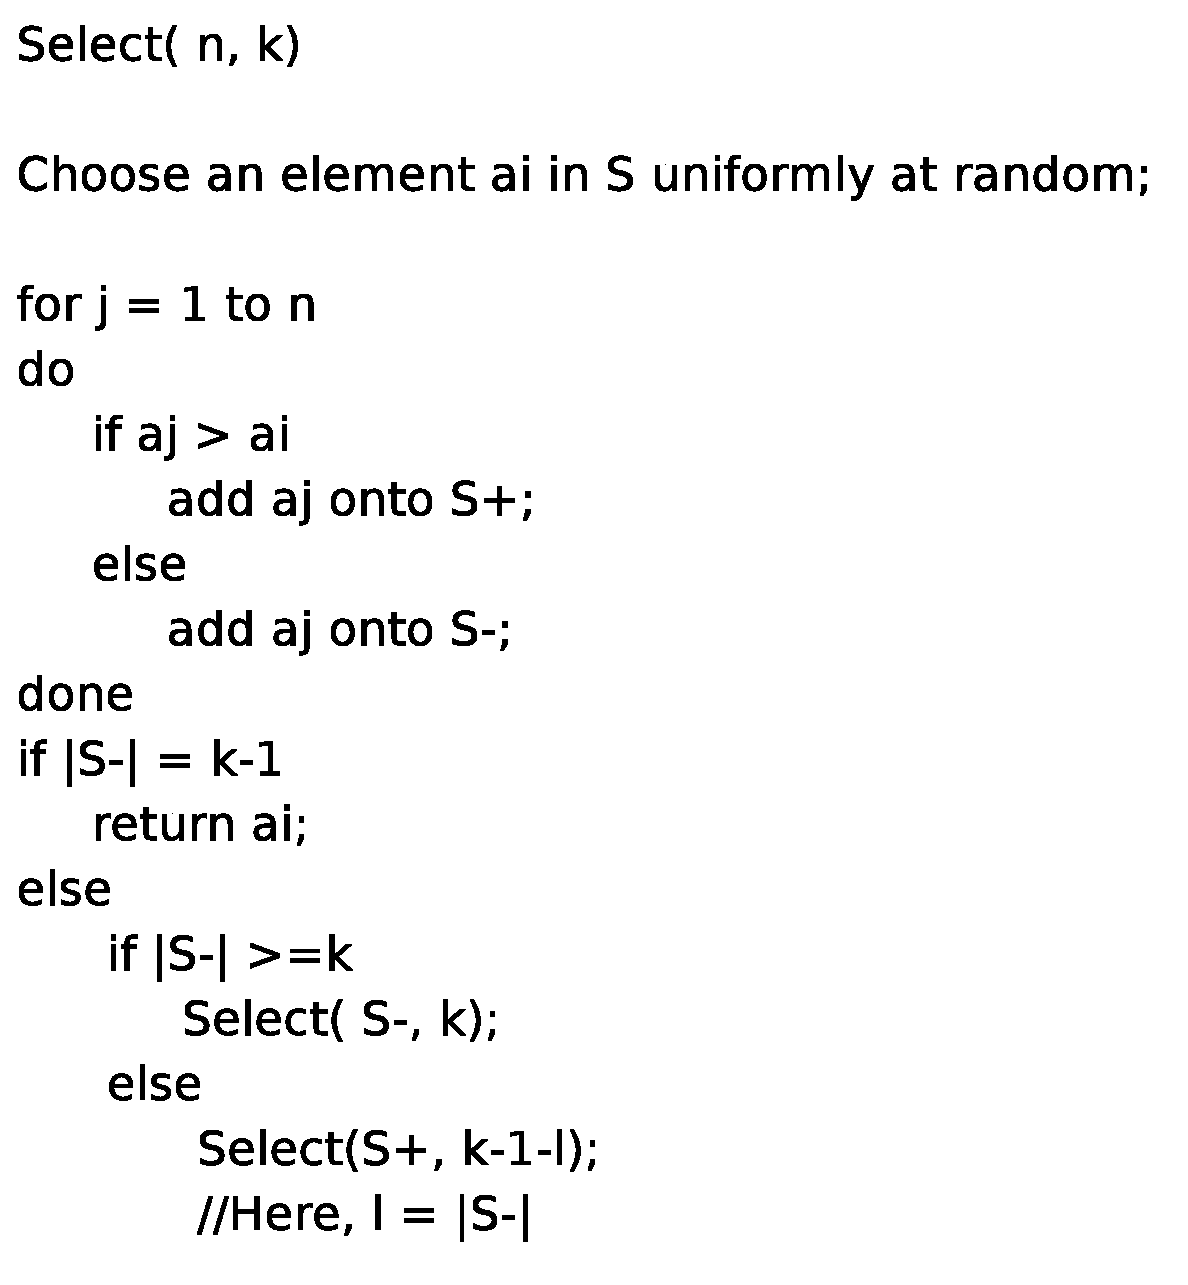
\includegraphics[width=2in]{L12-randomizedkmedian.eps}
 \end{figure}
 \begin{figure}
        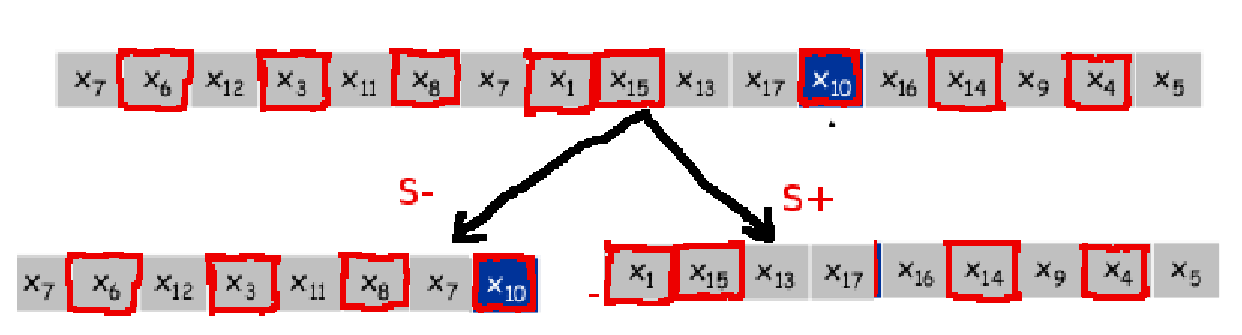
\includegraphics[width=3in]{L12-randomizedkmedianalgo.eps}
 \end{figure}


(Intuition: sloving an extension of the original problem, i.e., to find the $k$-th median. At first, an element $a_i$ is chosen to split $S$ into two parts $S^+=\{a_j: a_j \geq a_i\}$, and $S^-=\{a_j: a_j < a_i\}$. We can determine whether the $k$-th median is in $S^+$ or $S^-$. Thus, we perform iteration on ONLY one subset.)


Difficulty: how to choose the splitter? 
\begin{itemize}
 \item Bad choice: select the smallest element at each iteration. 
$T(n)=T(n-1)+O(n) = O(n^2)$
 \item Ideal choice: select the median at each iteration. 
$T(n)=T(\tfrac{n}{2})+O(n)=O(n)$
 \item Good choice: select a ``centered'' element $a_i$, i.e., $|S^+| \geq \epsilon n$, and $|S^-| \geq \epsilon n$ for a fixed $\epsilon > 0$. 
$T(n)\leq T( (1-\epsilon)n) + O(n) \leq cn+c(1-\epsilon)n+c(1-\epsilon)^2n+.... = O(n)$. 
\end{itemize}

e.g.: $\epsilon=\frac{1}{4}$: 
\begin{figure}
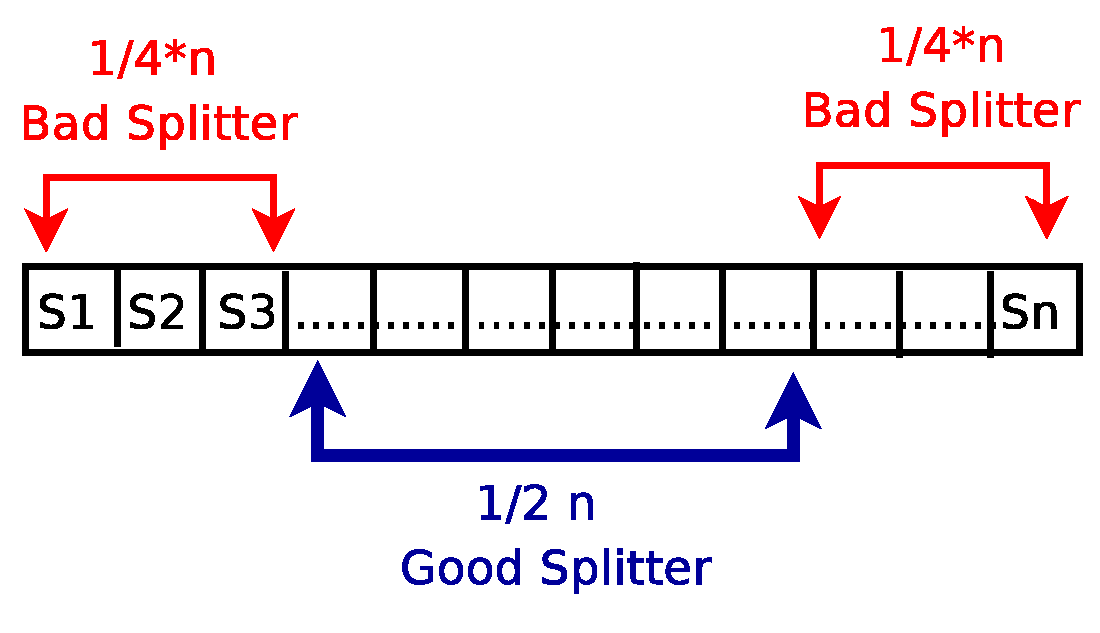
\includegraphics[width=2.5in]{L12-randomdcsplitter.eps}
\end{figure}

Key observation: if we choose a splitter $a_i \in S$ uniformly at random, it is easy to get a good splitter since a fairly large fraction of the elements are ``centered''. 

\begin{Theorem}
 The expected running time of Select(n,k) is $O(n)$.
\end{Theorem}
\begin{Proof}
 \begin{itemize}
  \item Let $\epsilon=\tfrac{1}{4}$. We'll say that the algorithm is in phase $j$ when the size of set under consideration is in $[n(\tfrac{3}{4})^{j-1}, n(\tfrac{3}{4})^{j}]$. 
  \item Let $X$ be the number of steps. And $X_j$ be the number of steps in phase $j$. Thus, $X=X_0+X_1+...$. 
  \item Consider the $j$-th phase. The probability to find a centered splitter is $\geq \tfrac{1}{2}$ since  at least half elements are centered. Thus, the expected number of iterations  to find a centered splitter is: $2$. 
  \item Each iteration costs $cn(\tfrac{3}{4})^j$ steps since there are at most $n(\tfrac{3}{4})^j$ elements in phase $j$. Thus,  $E(X_j)\leq 2 cn(\tfrac{3}{4})^j$.
  \item $E(X) = E(X_0 + X_1 + ....) \leq \sum_j 2cn (\tfrac{3}{4})^j \leq 8cn$.  
 \end{itemize}

\end{Proof}

}

\frame{
\frametitle{Hashing}
(See extra slides)
}


\end{document}
